\documentclass[border=3pt]{standalone}
\usepackage{amsmath}\usepackage{amssymb}
\usepackage{fontspec}\setsansfont{Arial}\renewcommand{\familydefault}{\sfdefault}
\usepackage{tikz}
\usetikzlibrary{arrows.meta,positioning,calc,fit,backgrounds,shapes.geometric}
\definecolor{titlegray}{HTML}{5F6B78}\definecolor{ent}{HTML}{7B8794}
\definecolor{fo}{HTML}{5AA9C4}\definecolor{ho}{HTML}{2E6B86}
\definecolor{inf}{HTML}{D98A3D}\definecolor{vio}{HTML}{9B86C4}
\definecolor{smac}{HTML}{2E8AA6}\definecolor{kgc}{HTML}{E7B15A}
\definecolor{fillteal}{HTML}{E3EEF2}\definecolor{fillamber}{HTML}{FBF0E2}
\definecolor{fillgrey}{HTML}{F1F3F5}\definecolor{fillviolet}{HTML}{EFEAF6}
\definecolor{inkmid}{HTML}{3D4751}\definecolor{distract}{HTML}{B3403A}
\begin{document}
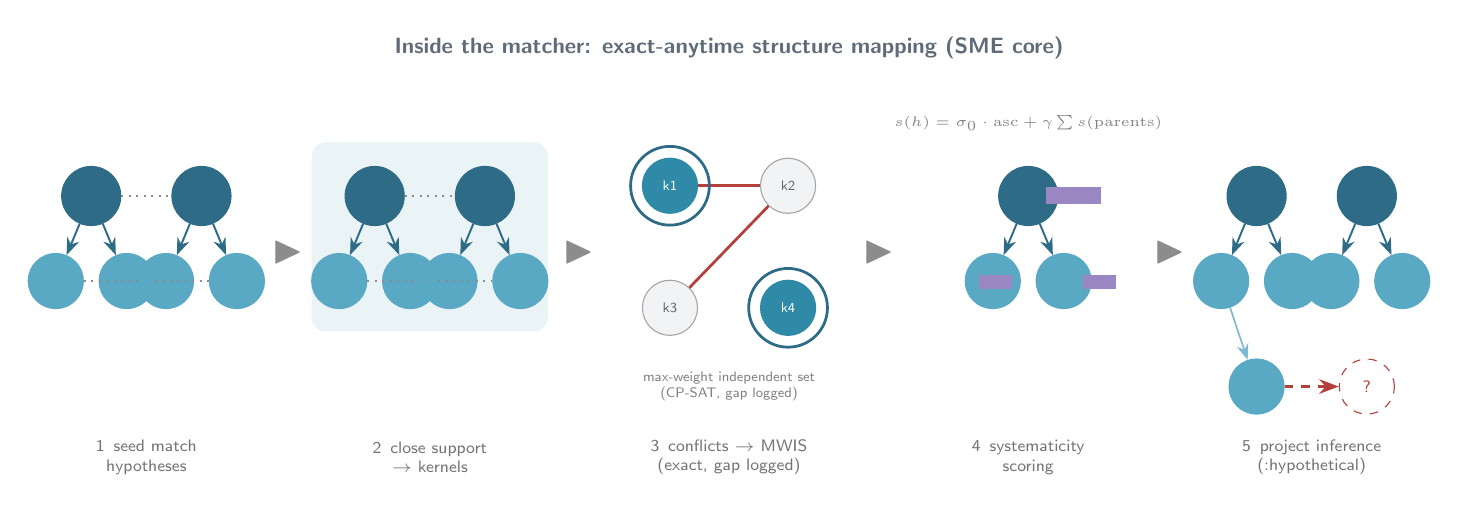
\begin{tikzpicture}[
  font=\sffamily,>=Stealth,
  ttl/.style={font=\sffamily\fontsize{8}{9}\selectfont\bfseries, color=titlegray, align=center},
  sub/.style={font=\sffamily\fontsize{6}{7}\selectfont, color=black!55, align=center},
  micro/.style={font=\sffamily\fontsize{5.2}{6}\selectfont, color=black!50, align=center},
  enode/.style={circle, draw=ent, fill=ent, text=white, font=\sffamily\fontsize{5.2}{6}\selectfont, inner sep=0pt, minimum size=6.5mm, align=center},
  fnode/.style={circle, draw=fo, fill=fo, text=white, font=\sffamily\fontsize{5.2}{6}\selectfont, inner sep=0pt, minimum size=7mm, align=center},
  hnode/.style={circle, draw=ho, fill=ho, text=white, font=\sffamily\fontsize{5.2}{6}\selectfont, inner sep=0pt, minimum size=7.5mm, align=center},
  pbox/.style={rounded corners=2pt, draw, align=center, inner sep=3pt, font=\sffamily\fontsize{6}{7}\selectfont},
  flowarr/.style={->, line width=0.7pt, color=black!55},
  horel/.style={->, line width=0.7pt, color=ho},
  forel/.style={->, line width=0.6pt, color=fo!80},
]
\node[ttl] at (9,5.6) {Inside the matcher: exact-anytime structure mapping (SME core)};
\node[hnode] (s1bt) at (0.9000000000000001,3.72) {};\node[fnode] (s1bl) at (0.4500000000000001,2.64) {};\node[fnode] (s1br) at (1.35,2.64) {};\draw[horel] (s1bt)--(s1bl); \draw[horel] (s1bt)--(s1br);\node[hnode] (s1tt) at (2.3,3.72) {};\node[fnode] (s1tl) at (1.8499999999999999,2.64) {};\node[fnode] (s1tr) at (2.75,2.64) {};\draw[horel] (s1tt)--(s1tl); \draw[horel] (s1tt)--(s1tr);\draw[dotted,line width=0.7pt,color=black!45] (s1bt)--(s1tt);\draw[dotted,line width=0.7pt,color=black!45] (s1bl)--(s1tl);\draw[dotted,line width=0.7pt,color=black!45] (s1br)--(s1tr);\begin{scope}[on background layer]\fill[smac!10,rounded corners=5pt] (3.7,2.0) rectangle (6.7,4.4);\end{scope}\node[hnode] (s2bt) at (4.5,3.72) {};\node[fnode] (s2bl) at (4.05,2.64) {};\node[fnode] (s2br) at (4.95,2.64) {};\draw[horel] (s2bt)--(s2bl); \draw[horel] (s2bt)--(s2br);\node[hnode] (s2tt) at (5.9,3.72) {};\node[fnode] (s2tl) at (5.45,2.64) {};\node[fnode] (s2tr) at (6.3500000000000005,2.64) {};\draw[horel] (s2tt)--(s2tl); \draw[horel] (s2tt)--(s2tr);\draw[dotted,line width=0.7pt,color=black!45] (s2bt)--(s2tt);\draw[dotted,line width=0.7pt,color=black!45] (s2bl)--(s2tl);\draw[dotted,line width=0.7pt,color=black!45] (s2br)--(s2tr);\node[circle,draw=smac,fill=smac,text=white,minimum size=7mm,font=\sffamily\fontsize{5}{6}\selectfont] (k1) at (8.25,3.85) {k1};\node[circle,draw=black!35,fill=fillgrey,text=black!60,minimum size=7mm,font=\sffamily\fontsize{5}{6}\selectfont] (k2) at (9.75,3.85) {k2};\node[circle,draw=black!35,fill=fillgrey,text=black!60,minimum size=7mm,font=\sffamily\fontsize{5}{6}\selectfont] (k3) at (8.25,2.3) {k3};\node[circle,draw=smac,fill=smac,text=white,minimum size=7mm,font=\sffamily\fontsize{5}{6}\selectfont] (k4) at (9.75,2.3) {k4};\draw[line width=1pt,color=distract] (k1)--(k2); \draw[line width=1pt,color=distract] (k2)--(k3);\node[draw=ho,line width=1pt,circle,minimum size=10mm] at (k1) {}; \node[draw=ho,line width=1pt,circle,minimum size=10mm] at (k4) {};\node[micro] at (9.0,1.3) {max-weight independent set\\(CP-SAT, gap logged)};\node[hnode] (s4t) at (12.8,3.72) {};\node[fnode] (s4l) at (12.350000000000001,2.64) {};\node[fnode] (s4r) at (13.25,2.64) {};\draw[horel] (s4t)--(s4l); \draw[horel] (s4t)--(s4r);\fill[vio] (13.020000000000001,3.62) rectangle ++(0.7,0.22);\fill[vio] (12.180000000000001,2.54) rectangle ++(0.42,0.18);\fill[vio] (13.5,2.54) rectangle ++(0.42,0.18);\node[micro] at (12.8,4.65) {$s(h)=\sigma_0\cdot\mathrm{asc}+\gamma\sum s(\mathrm{parents})$};\node[hnode] (s5bt) at (15.7,3.72) {};\node[fnode] (s5bl) at (15.25,2.64) {};\node[fnode] (s5br) at (16.15,2.64) {};\draw[horel] (s5bt)--(s5bl); \draw[horel] (s5bt)--(s5br);\node[fnode] (s5bc) at (15.7,1.3) {}; \draw[forel] (s5bl)--(s5bc);\node[hnode] (s5tt) at (17.099999999999998,3.72) {};\node[fnode] (s5tl) at (16.65,2.64) {};\node[fnode] (s5tr) at (17.549999999999997,2.64) {};\draw[horel] (s5tt)--(s5tl); \draw[horel] (s5tt)--(s5tr);\node[circle,draw=distract,dashed,fill=white,text=distract,minimum size=7mm,font=\sffamily\fontsize{6}{7}\selectfont] (s5q) at (17.099999999999998,1.3) {?};\draw[->,dashed,line width=0.9pt,color=distract] (s5bc)--(s5q);\node[sub] at (1.6,0.4) {1\, seed match\\hypotheses};\node[sub] at (5.2,0.4) {2\, close support\\$\rightarrow$ kernels};\node[sub] at (9.0,0.4) {3\, conflicts $\rightarrow$ MWIS\\(exact, gap logged)};\node[sub] at (12.8,0.4) {4\, systematicity\\scoring};\node[sub] at (16.4,0.4) {5\, project inference\\(:hypothetical)};\node[color=black!45,font=\Large] at (3.4000000000000004,3.0) {$\blacktriangleright$};\node[color=black!45,font=\Large] at (7.1,3.0) {$\blacktriangleright$};\node[color=black!45,font=\Large] at (10.9,3.0) {$\blacktriangleright$};\node[color=black!45,font=\Large] at (14.6,3.0) {$\blacktriangleright$};
\end{tikzpicture}
\end{document}
